
\chapter{Introduction}\label{s:introduction}
Humidity, defined as the amount of water vapor present in air, is an important environmental parameter that impacts many aspects of daily life as well as various industrial processes, agricultural production and scientific applications. Precise measurement of humidity and related environmental descriptors is therefore necessary across a range of fields \autocite{korotcenkovHandbookHumidityMeasurement2018}.

In daily life, humidity most importantly affects human health and comfort. High humidity exacerbates conditions such as asthma, allergies, and arthritis for affected individuals \autocite{andersenAsthmaIndoorEnvironment1986, aikmanAssociationArthritisWeather1997}. Thermal comfort is also closely tied to humidity levels in addition to temperature, resulting in relative humidity as the most commonly used parameter for the moisture concentration in the air \autocite{alsmoVentilationRelativeHumidity2014}. Besides health and comfort, humidity influences the effectiveness of heating and cooling systems as well as the likelihood of mold growth \autocite{blockHumidityRequirementsMold1953}.

Industrially and agriculturally, humidity control is critical for manufacturing processes in sectors such as food, pharmaceuticals, textiles, and electronics. Stability and quality of products rely heavily on ambient humidity during production. Insufficient humidity levels can cause issues like cracking, fragility, and degradation of products that naturally absorb moisture \autocite{osenbachCorrosioninducedDegradationMicroelectronic1996}. For example, wood products may crack or warp, food items may lose weight or texture \autocite{wangReviewLongtermEffects2021}. Excessive amounts of water vapor may degrade foods or hygroscopic pharmaceuticals or lead to failures in chemical processes \autocite{blockHumidityRequirementsMold1953}. Proper humidity control therefore enables a reliable and quality-controlled production of materials and goods.

Scientifically, accurate humidity data is vital in meteorology to predict and model weather patterns, precipitation, cloud formation and more \autocite{heerwaardenRelativeHumidityIndicator2008}. Environmental sciences additionally track humidity over landscapes and ecosystems as an indicator of overall health. Botany research also requires monitored humidity in order to analyze and compare plant parameters such as growth rates, physiology or disease resistance under controlled environmental conditions \autocite{talbottRelativeHumidityKey2003}.

\section{Aim of this work}
Due to the aforementioned importance of reliable and precise quantification of humidity in countless numbers of different environments, a vast variety of humidity sensors has been developed over the course of history. While various humidity measurement technologies are currently used, they employ different advantages and drawbacks in key parameters such as accuracy, response time, stability, and cost. 

One single, but due to its accuracy very important measurement concept is the dew point mirror hygrometer, which determines the humidity based on the determination of the so-called dew point temperature using a thermo-optical architecture, as thoroughly described in the following sections of this work. The aim of this thesis is to investigate methods to improve the cost characteristic of accurate humidity measurement through the development of a highly integrated dew-point hygrometer, using components that allow for a downscaling and cost-cutting of conventional dew point hygrometers as well as to evaluate the effect on measurement accuracy. 

The sensor demonstrates improved performance across key metrics necessary for reliable humidity monitoring. Widespread adoption of the sensor would therefore benefit applications across daily life, industry, and science through more precise humidity measurements.


\chapter{Background}\label{s:background}
Before introducing and discussing the investigated concepts for humidity measurements, it is important to have a solid grasp of the meaning of humidity and the fundamental physics that govern it. The next sections explain the key definitions of humidity, specifically with regards to measurement purposes, as well as the main parameters used to describe humidity levels. To provide some context, a quick overview of the most widely-used approaches to measuring humidity is also given.

\section{Physics of humidity and evaporation}
Generally speaking, humidity refers to the amount of water vapor, that is the gaseous phase of water below its critical temperature, present in a gas mixture such as air \autocite{greenPerryChemicalEngineers2019}.

\begin{wrapfigure}{r}{0.43\textwidth}
    \centering
    \def\svgwidth{0.4\textwidth}
    \input{drawings/evaporation.pdf_tex}
    \caption{Process of evaporation.}
\end{wrapfigure}

Water molecules are polar, with a partially positive charge on the hydrogen atoms and a partially negative charge on the oxygen atom. This allows the hydrogen atom of one water molecule to form a weak attraction to the oxygen atom of another water molecule, called a hydrogen bond. Due to the temperature-dependant kinetic energy of the water molecules, hydrogen bonds between them are continually breaking and reforming. With increasing temperatures, more bonds are broken than formed, leading to evaporation which is invisible for the human eye. Only as temperatures increase so much, that the water vapor pressure exceeds the atmospheric pressure, the evaporation becomes evident due to the boiling of the liquid water, leading to visible bubbles as the density of water vapor is much less than that of liquid water.

\subsection{Equilibrium vapor pressure}\label{c:equilibriumvaporpressure}
As a volume contains an increasing amount of water vapor, the partial pressure exerted by said vapor increases. If the water vapor pressure reaches the saturation vapor pressure, also called equilibrium vapor pressure, the water vapor is in a thermodynamic equilibrium with its condensed phase, meaning there is a macroscopic balance between evaporation and, depending on the phase transition, condensation or sublimation. In an isothermal process, even in case of compression the vapor pressure will remain constant for a certain decrease in the gas volume through an increased rate of condensation, the liquid and vapor phase are in coexistence.
The equilibrium water vapor pressure is defined over a flat surface of pure liquid water, which is relevant as the point of equilibrium is different depending on the surface tension of the water molecules \autocite{babinWaterVaporMyths,iribarneThermodynamicProcessesAtmosphere1981}

Tiny water droplets consisting of only a few water molecules exhibit significantly less surface tension due to their curvature, hence the partial vapor pressure needs to exceed the equilibrium vapor pressure in such a case in order to condensate and to form droplets, leading to a relative humidity of well over \qty{100}{\%}. This phenomenon is referred to as supersaturation, however it is usually only seen to a certain extent in upper atmosphere. In practice, small particles called condensation nuclei, which have a size of a few hundred nanometers, help the formation of water droplets by providing a sufficiently flat surface for molecules to stick to and limit the influence of the curvature effect in the formation of clouds, fog, etc. \autocite{iribarneThermodynamicProcessesAtmosphere1981}.

On the other hand, the partial pressure of water vapor in the atmosphere may not reach equilibrium vapor pressure due to the presence of hygroscopic nuclei and the process of deliquescence. Hygroscopic nuclei are small particles in the atmosphere that readily attract and absorb water molecules from the surrounding air, such as salt particles like sodium chloride and calcium chloride. These hygroscopic particles undergo a process called deliquescence where they dissolve by absorbing moisture from the air once the relative humidity reaches a certain level known as the deliquescence point. The moisture gets trapped in a thin coating of solution around the particles and causes the partial pressure of water vapor to drop below the equilibrium vapor pressure determined by the ambient temperature. As seen later, this effect can be used to create environments with a controlled humidity for calibration of humidity sensors.

\subsection{Clausius–Clapeyron relation and common approximations}
The saturation vapor pressure is not constant but highly depends on the temperature according to the Clausius–Clapeyron relation. Using the ideal gas law, which neglects the volume of the gas particles as well as the attracting and repulsive forces between themselves, the relation can be approximated to:
\begin{equation}\label{e:clausius}
    \frac{\mathrm{d}p_s}{\mathrm{d}T} = \frac{L_v(T) p_s}{R_v T^2},
\end{equation}
where
$p_s$: saturation vapor pressure of water, 
$T$: temperature, 
$L_v$: specific latent heat of evaporation, 
$R_v$: gas constant of water vapor \autocite{iribarneThermodynamicProcessesAtmosphere1981}.

Latent energy is the energy needed to be supplied or extracted in order to change the phase of a substance without changing the temperature or pressure. As it is temperature dependent itself, the differential equation of Clausius-Clapeyron is computationally expensive to solve. The need for analytical expressions as well as mismatches of the theoretical equation compared to empiric measurements due to the deviations of the ideal gas law compared to the real behaviour of gas have lead to the development of approximations in explicit forms, many of which are improvements of the early August-Roche-Magnus equation, or shorthand Magnus equation, from 1844 \autocite{alduchovImprovedMagnusForm1997}.

Following formula is a Magnus-type equation with coefficients from Sonntag (1990), as proposed in the Guide to Instruments and Methods of Observations, published by the \gls{WMO} (2018):
% formatting: https://tex.stackexchange.com/questions/453195/how-to-align-subequations-when-each-subequation-has-multiple-lines
\begin{subequations}
\begin{align}
    p_s &= 6.112 \exp\left(\frac{17.62 \cdot T}{T + 243.12}\right) & \text{(over water)} \\
    p_s &= 6.112 \exp\left(\frac{22.46 \cdot T}{T + 272.62}\right) & \text{(over ice)}
\end{align}
\end{subequations}
where 
$p_s$: water vapor saturation pressure in \unit{\hecto\pascal}, 
$T$: temperature in \unit{\celsius} \autocite{worldmeteorologicalorganizationMeasurementMeteorologicalVariables2018}.


\begin{figure}[h]
    \centering
    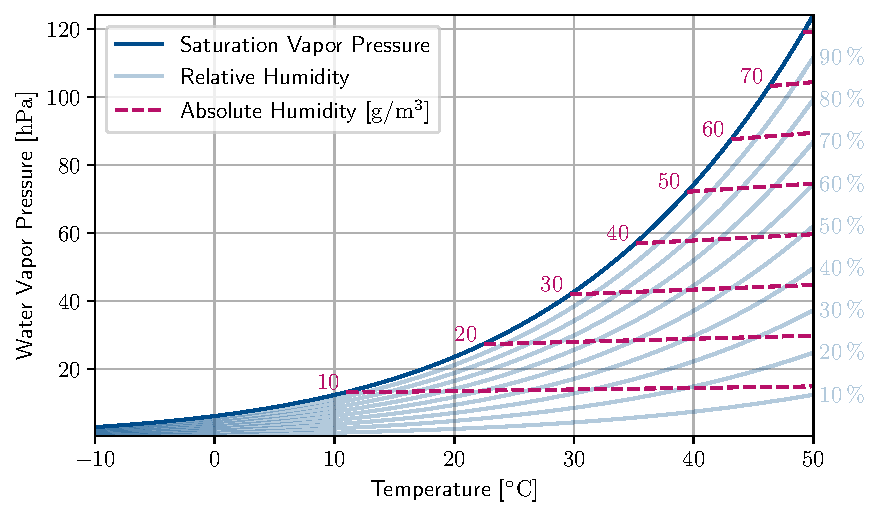
\includegraphics[width=1\textwidth]{graphs/saturation_pressure_chart.pdf}
    \caption{Water vapor saturation pressures based on \cref{e:sonntag}.}
\end{figure}

Standard laboratories such as the german \gls{PTB} or the british \gls{NPL} use the formulas of Sonntag (1994), based on Wexlers' formulas from 1976 \autocite{dirksenEinheitlichesBerechnungsverfahrenFuer2019}:
\begin{subequations}\label{e:sonntag}
\begin{align}
\begin{split}
    \ln{p_s} &= \begin{aligned}[t]
    &\mathrlap{-\frac{6096.9385}{T} + 16.635794 - \num{2.711193e-2} \cdot T} \\
    &+ \num{1.673952e-5} \cdot T^2 + 2.433502 \cdot \ln(T)) & \text{(over water)}
    \end{aligned}
\end{split}
\label{e:transverse_straincore} 
\\
\begin{split}
    \ln{p_s} &= \begin{aligned}[t]
    &\mathrlap{-\frac{6024.5282}{T} + 24.721994 - \num{1.0613868E-2} \cdot T} \\
    &+ \num{-1.3198825E-5} \cdot T^2 + -0.49382577 \cdot \ln(T)) & \text{(over ice)}
    \end{aligned}
\end{split}
\label{e:transverse_straincoore} 
\end{align}
\end{subequations}
where 
$p_s$: water vapor saturation pressure in \unit{\pascal}, 
$T$: temperature in \unit{\kelvin}.

The shown equations differentiate between the surface pressure over ice and that over liquid water. This is due to ice producing a lower vapor pressure than liquid water, with deviations of up to \qty{0.28}{\hecto\pascal} at \qty{-15}{\celsius}.

Common to all equations is that they are valid for a pure phase of water vapor, neglecting the influence of the atmosphere. Therefore pressure- and temperature-dependent enhancement factors have been developed and described by Goff (1949) and Sonntag (1982). 
Due to the very weak influence of the temperature, the approximated formula for surface measurements can be reduced to its pressure-dependent parts as stated in in the WMO Guide (2018) \autocite{buckNewEquationsComputing1981,worldmeteorologicalorganizationMeasurementMeteorologicalVariables2018}:
\begin{equation}
    f(p_{atm}) = 1.0016 + \num{3.15e-6} \cdot p_{atm} - 0.074p_{atm}^{-1}
\end{equation}
where
$f$: enhancement factor, 
$p$: atmospheric pressure in \unit{\pascal}.

At sea level, this results in a factor of approximately \num{1.005} to be used for determining the most precise value of the water vapor saturation pressure at a given temperature.

\subsection{Dew point}
As we have already seen, the equilibrium vapor pressure depends mainly on the temperature of the water molecules. This leads to the definition of another term in the context of humidity called dew point temperature. If the temperature of water vapor decreases, the water vapor becomes saturated and condensation starts to take place. The resulting temperature is called dew point temperature. In more technical terms, the dew point describes the temperature, at which the water vapor of a humid gas starts to condense, and is dependent on the partial water vapor pressure.
% https://www.wufi-forum.com/viewtopic.php?t=1615

\section{Parameters of humidity}
Following the information given in the previous section, there are a few different ways to quantify and describe humidity \autocite{greenPerryChemicalEngineers2019}:
\begin{itemize}
    \item \textbf{Absolute humidity} or volumetric humidity is defined as the mass of water vapor per unit volume of the gas mixture: 
    \begin{equation}
    AH = \frac{m_w}{V}
    \end{equation}
    
    It is typically expressed as \unit{g\per m^3} for air and gives a direct measure of the actual amount of water vapor present.
    \item  \textbf{Relative humidity} is expressed as a percentage of the partial vapor pressure in relation to the equilibrium vapor pressure or in other words, relative humidity compares the current absolute humidity to the maximum possible absolute humidity at a given temperature. As seen in the last section, the maximum absolute humidity depends on the equilibrium vapor pressure of water at a given temperature and atmosphere.
    \begin{equation}\label{e:rh}
    RH(p, T) = \qty{100}{\%} \cdot \frac{p}{p_s(T)},
    \end{equation}
    where $RH$: relative humidity, $p$: partial water vapor pressure, $p_s$: saturation water vapor pressure.

    The conversion from absolute humidity to relative humidity for a known temperature can be performed using the molar form of the ideal gas law and the specific gas constant of water $R_v$:
    \begin{equation}
    p = \frac{m_w}{V} R_v T
    \end{equation}
    \item \textbf{Specific humidity} is defined as the mass of vapor per unit mass of gas-vapor mixture.
    \item \textbf{Dew point temperature} is the temperature at which a given mixture of water vapor and air becomes saturated on cooling. In terms of water vapor pressure, this phenomenon can be expressed as partial water vapor pressure $p = p_s(T_{dew})$, hence for a known dew point temperature, \cref{e:rh} can be written as:
    \begin{equation}
    RH = \qty{100}{\%} \cdot \frac{p}{p_s(T)} = \qty{100}{\%} \cdot \frac{p_s(T_{dew})}{p_s(T)}
    \end{equation}
    
\end{itemize}

\section{Types of hygrometers}\label{s:hygrometertypes}
Over the centuries, a large variety of principles has been used in order to determine the amount of moisture within different environments. Following sections briefly describe the most relevant transduction principles and commonly used sensors. For a more detailled and comprehensive analysis, please refer to \autocite{fontesHumiditySensors2005,korotcenkovHandbookHumidityMeasurement2018,korotcenkovHandbookHumidityMeasurement2019,rittersmaRecentAchievementsMiniaturised2002a}.

\subsection{Gravimetric hygrometers}
Gravimetric hygrometers are considered to be the first sensors developed by mankind for determining the humidity. The principle is very simple: A moisture-absorbent, also called hygroscopic, material, such as wool, cotton or hair is first weighed in a reference environment and thereafter measured after exposure to dry or humid air. The measured unit is the mass ratio of the used medium, which thereby indicates the level of humidity. The intended use of such sensors was to visualize and predict changes in weather conditions. While today this method is not broadly used, it still serves for calibration purposes of other humidity sensors, as its accuracy is greatly affected by the surroundings such as air convection in the case of temperature differences between the sensor and its environment, and hence in terms of humidity measurements mostly limited to laboratory usage.

\subsection{Mechanical hygrometer}
Mechanical hygrometers also count as an early method for sensing humidity, with one of the first being the human hair hygrometer invented by Horace Bénédict de Saussure. This class of sensors is based on the principal of dimensional changes due to varying humidity, in case of the hair hygrometer being an expansion or shrinkage of the hair. Hair consists mainly of keratin, a protein filament, which is held together in a helical structure by hydrogen bonds. In case of exposure to moisture, the hydrogen bonds break, allowing the coil of keratin fibers to stretch and the hair to lengthen. This effect is entirely reversible if the moisture is extracted from the hair. The total amount of change in length depends on the type of hair and varies from human to human but can be generally quantified as a maximum change in length of \qty{2}{\%} to \qty{2.5}{\%} for a change in relative humidity from \qty{0}{\%} to \qty{100}{\%}. The accuracy is typically within \qty{5}{\%} to \qty{10}{\%} relative humidity, with potentially more accurate results in environments with room temperature and with relative humidities of around \qty{40}{\%} to \qty{60}{\%}. Other mechanical types of hygrometers are using other types of materials or laminates in order to improve uniformity or accuracy.

\subsection{Psychrometers}
The psychrometer, also known as wet-bulb/dry-bulb hygrometer, is a very commonly used method for humidity sensing. The name derives from the greek word "psychro", which translates to "cold". The principle of operation is the comparison of two matching thermometers, that of a dry bulb thermometer and that of a wet bulb thermometer. As described by \cref{e:clausius}, the process of evaporation requires an amount of heat equal to the latent heat of vaporization in order to change the phase from liquid to vapor. If one thermometer is enclosed in a porous, hygroscopic medium that draws water from a reservoir by the capillary effect, it will measure a lower temperature due to said extraction of heat. The difference between dry-bulb and wet-bulb temperature is called "wet-bulb depression" and can be used to determine the relative humidity according to Sprung's formula:
\begin{equation}
    \begin{split}
        p & = p_s(T_{wet}) - A \cdot P \cdot (T_{wet} - T_{dry}) \\
        \iff RH & = \qty{100}{\%} \cdot \frac{p_s(T_{wet}) - A \cdot P \cdot (T_{wet} - T_{dry})}{p_s(T_{dry})},
    \end{split}
\end{equation}
where $A$: psychrometer coefficient, $P$: total pressure

\subsection{(Mirror based) dew point sensors}
Dew Point Sensors are based on the effect of condensation or sublimation in case of a cooling of the water vapor. They are used to measure the dew point temperature of a gas, which is the temperature at which water vapor in the gas condenses into liquid water. They work on the principle of cooling a surface such as a mirror until condensation forms on it. The temperature at which this condensation begins is recorded as the dew point temperature. Dew point hygrometers were invented in 1783 by Swiss physicist and geologist Horace Bénédict de Saussure. The basic structure consists of a polished metal mirror connected to a cooling system. The mirror is cooled while the humid air flows over it. An optical system detects when condensation first forms on the mirror by changes in reflectivity. The temperature of the mirror is precisely controlled through feedback circuits to maintain equilibrium between condensation forming and evaporating on the mirror surface. This temperature is measured and recorded as the dew point. Modern chilled-mirror dew point hygrometers use advanced optics and electronics to precisely detect the onset of condensation on the mirror. They are considered among the most accurate instruments for humidity measurement \autocite{korotcenkovHandbookHumidityMeasurement2019}.

\subsection{Capacitive sensors}\label{s:capacitive_sensors}
Capacitive hygrometers operate on the principle that the dielectric constant of hygroscopic materials changes as they adsorb moisture from the surrounding environment. This alters the capacitance between two conductive plates separated by the dielectric. By measuring this change in capacitance, the relative humidity can be determined. In a typical structure, the sensor consists of a thin film of polymer or metal oxide like aluminum oxide, sandwiched between two electrodes coated on a glass or ceramic substrate. When water vapor is absorbed by the dielectric, its dielectric constant increases, resulting in increased capacitance between the plates according to the equation:
\begin{equation}
    C = \epsilon_0 \epsilon_r \frac{A}{d},
\end{equation}
where $C$: capacitance, $\epsilon_0$: vacuum permittivity constant, $\epsilon_r$: relative permittivity, $A$: plate area, $d$: plate distance.

The change in capacitance can be detected using a variety of readout circuits based on different parameter changes with respect to capacitance, such as voltage, phase shift, duty cycle or frequency \autocite{hafizi-mooriCapacitanceReadoutCircuits2016}. While capacitive senors are the most commonly used sensors today, due to their good performance in typical environments, low cost and small size, they suffer from long-term drift due to degradation in used materials and hence need to be calibrated regularly \autocite{chenHumiditySensorsReview2005,korotcenkovHandbookHumidityMeasurement2019}.

